% Fermentation Model
% Design a high level diagram of the fermentation process, including the lifespan of cells using tikz
\documentclass{documentclass{standalone }}
\usepackage{tikz}
\begin{document}
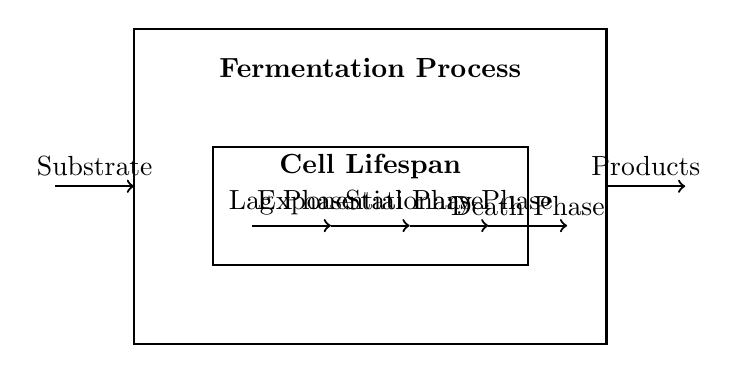
\begin{tikzpicture}
    % Draw the main process box
    \draw[thick] (0,0) rectangle (6,4);
    \node at (3,3.5) {\textbf{Fermentation Process}};
    
    % Draw the input and output arrows
    \draw[->, thick] (-1,2) -- (0,2) node[midway, above] {Substrate};
    \draw[->, thick] (6,2) -- (7,2) node[midway, above] {Products};
    
    % Draw the cell lifespan diagram inside the process box
    \draw[thick] (1,1) rectangle (5,2.5);
    \node at (3,2.25) {\textbf{Cell Lifespan}};
    
    % Draw the stages of cell lifespan
    \draw[->, thick] (1.5,1.5) -- (2.5,1.5) node[midway, above] {Lag Phase};
    \draw[->, thick] (2.5,1.5) -- (3.5,1.5) node[midway, above] {Exponential Phase};
    \draw[->, thick] (3.5,1.5) -- (4.5,1.5) node[midway, above] {Stationary Phase};
    \draw[->, thick] (4.5,1.5) -- (5.5,1.5) node[midway, above] {Death Phase};
\end{tikzpicture}
\end{document}